\documentclass[fontsize=12pt]{article}
\usepackage[utf8]{inputenc}
\usepackage[T1]{fontenc}
\usepackage[german]{babel}
\usepackage{amsmath}
\usepackage{amsthm}
\usepackage{amsfonts}
\usepackage{amssymb}
\usepackage{minted}
\usepackage{tikz}
\usepackage{pgfplots}
\usepackage[top=2cm, bottom=2cm, left=2cm, right=2cm, headheight=1.5cm]{geometry}
\usepackage{fancyhdr}
\usepackage{mdframed}
\usemintedstyle{emacs}

\definecolor{purp}{HTML}{9A72AC}
\definecolor{re}{HTML}{FC6255}
\definecolor{gre}{HTML}{83C167}
\definecolor{blu}{HTML}{58C4DD}
\definecolor{shadecolor}{rgb}{0.85,0.85,0.85}
\definecolor{bg}{rgb}{0.95,0.95,0.95}
\setlength{\parindent}{0em} 

\BeforeBeginEnvironment{minted}{\begin{mdframed}[linewidth =2 ,backgroundcolor=bg , linecolor=black, linewidth=0.5]}
\AfterEndEnvironment{minted}{\end{mdframed}}

\newenvironment{defi}[1]{
    \begin{shaded*}
    \textbf{Definition #1} \\
}{
    \end{shaded*}
}

\newcommand{\bsp}{\textbf{Beispiel}:}
%\newcommand{\task}{\textbf{Aufgabe}:}

\newcommand{\bol}[1]{\textbf{#1}}
\newcommand{\q}[1]{\glqq #1\grqq}
\newcommand{\DODO}[1]{\textbf{\textcolor{red}{DODO:}} #1 \\ \begin{center}\includegraphics[scale=0.2]{../../media/dodo.jpg} \end{center}}

\newenvironment{task}[1]{
    \begin{shaded*}
    \textbf{Aufgabe #1}:
}{
    \end{shaded*}
}



\fancypagestyle{firstpage}{
    \setlength{\headheight}{2.5cm}
    \setlength{\footskip}{0.25cm}
    \pagestyle{fancy}
    \renewcommand{\headrulewidth}{0.4pt}
    \fancyhf{}
    \fancyhead[L]{\LARGE\textbf{Aggregation und Referenzen}}
    \fancyhead[R]{\Large \textbf{Datum:} \hspace{2cm}}
    \fancyfoot[C]{\thepage}
}
\begin{document}
\thispagestyle{firstpage}
\setlength{\headsep}{12pt}
Neben Arrays ist es ein Wesentliches Ziel dieser Jahrgangsstufe, dass in Projekten mehrere Klassen verwendet werden (in kleinerer Form kam dies bereits in der neunten Klasse bei Klassendiagrammen vor!). \\
Damit Objekte verschiedener Klassen einfacher verknüpft werden können, werden sie häufig als Attribute angelegt - bisher waren Attribute hauptsächliche primitive Datentypen wie boolean, int oder double (String war schon die ganze Zeit eine Ausnahme!). \\
Zunächst ein anschaulicheres Beispiel: häufig \q{bestehen} Objekte hauptsächlich aus anderen Objekten (zumindest in der verwendeten Modellierung). Wollen wir beispielsweise ein Stickeralbum modellieren, benötigen wir zwei Klassen, eine für das Album und eine für einen einzelnen Sticker, man kann sagen: das Stickeralbum \textbf{enthält} die Sticker (das entspricht auch der Realität relativ gut!). \\
Im Fachbegriff heißt so eine \q{enthält}-Beziehung \textbf{Aggregation}. Im Objektdiagramm sähe das z.B. so aus: 
\begin{center}
    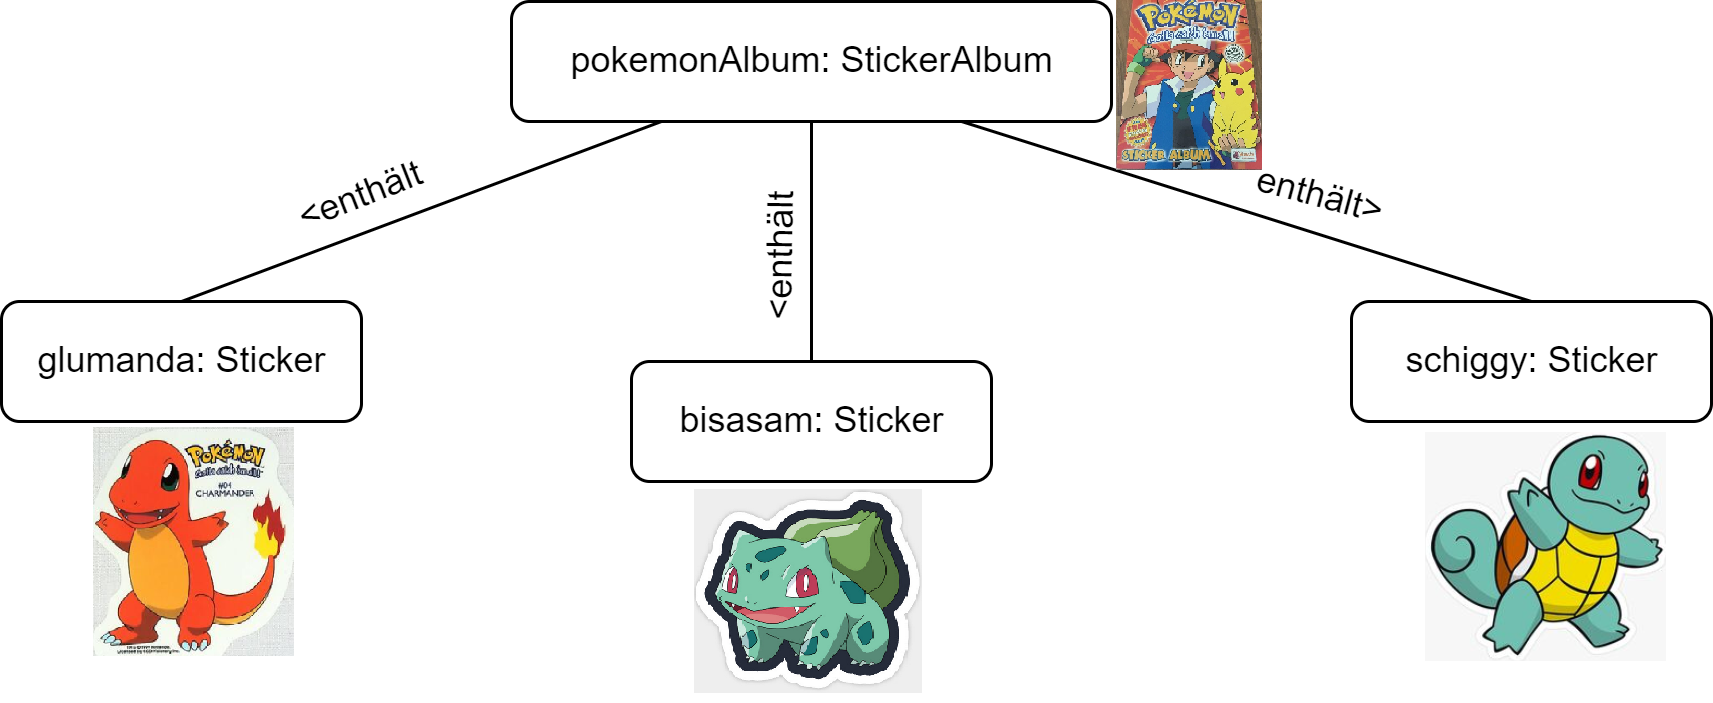
\includegraphics[scale=0.35]{media/obj_diagramm_album.png}
\end{center}
Im Klassendiagramm würde dies mit einem anderen Pfeil markiert werden:
\begin{center}
    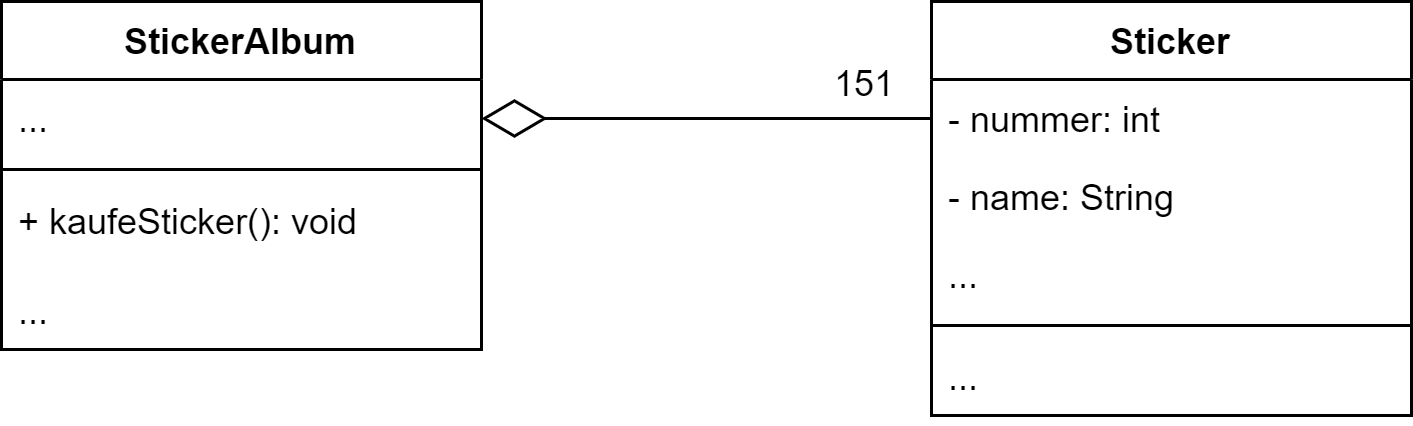
\includegraphics[scale=0.20]{media/class_diagram_album.png}
\end{center}
Ein StickerAlbum besteht also aus 151 Objekten vom Typ Sticker. Die \textbf{Multiplizität} $1$ beim StickerAlbum wird in der Regel weggelassen. Aggregationen werden - wie viele \q{Verbindungen} zwischen Klassen - mit Attributen realisiert. Vereinfachen wir unser Beispiel weiter und nehmen an, dass es nur drei Sticker gibt, dann könnte eine grundlegendeImplementierung des Stickeralbums so aussehen: 
\begin{minted}{java}
public class StickerAlbum {
    private Sticker glumanda;
    private Sticker bisasam;
    private Sticker schiggy;

    public StickerAlbum() {
        bisasam = new Sticker(1, "Bisasam");
        glumanda = new Sticker(4, "Glumanda");
        schiggy = new Sticker(7, "Schiggy");
    }
}
\end{minted}
Dabei wird - wie schon beim Array - mit dem Schlüsselwort \textbf{new} neue Objekte der Klasse Sticker erzeugt. (Man spricht auch von \textbf{Instanziierung)}. \\
\begin{minted}{java}
public class Sticker() {
    int nummer;
    String name;
    public Sticker(int nummer, int name) {
        this.nummer = nummer;
        this.name = name;
    }
}
\end{minted}
\vspace{2mm}
\textbf{Wichtig:} Die Sticker-Objekte sind nicht wirklich im StickerAlbum-Objekt \q{enthalten} im Sinne von: im Speicher stehen sie \q{ineinander}. Vielmehr ist die deklarierte Variable ein Zeiger (Fachbegriff: \textbf{Referenz}), die auf den Ort im Speicher verweist, an dem die eigentlichen Daten abgelegt sind - noch genauer gesagt: auf die Adresse der ersten Speicherzelle, die für das erzeugte Objekt verwendet wird. (im Folgenden noch mit Objektkarten veranschaulicht): \\
\begin{center}
    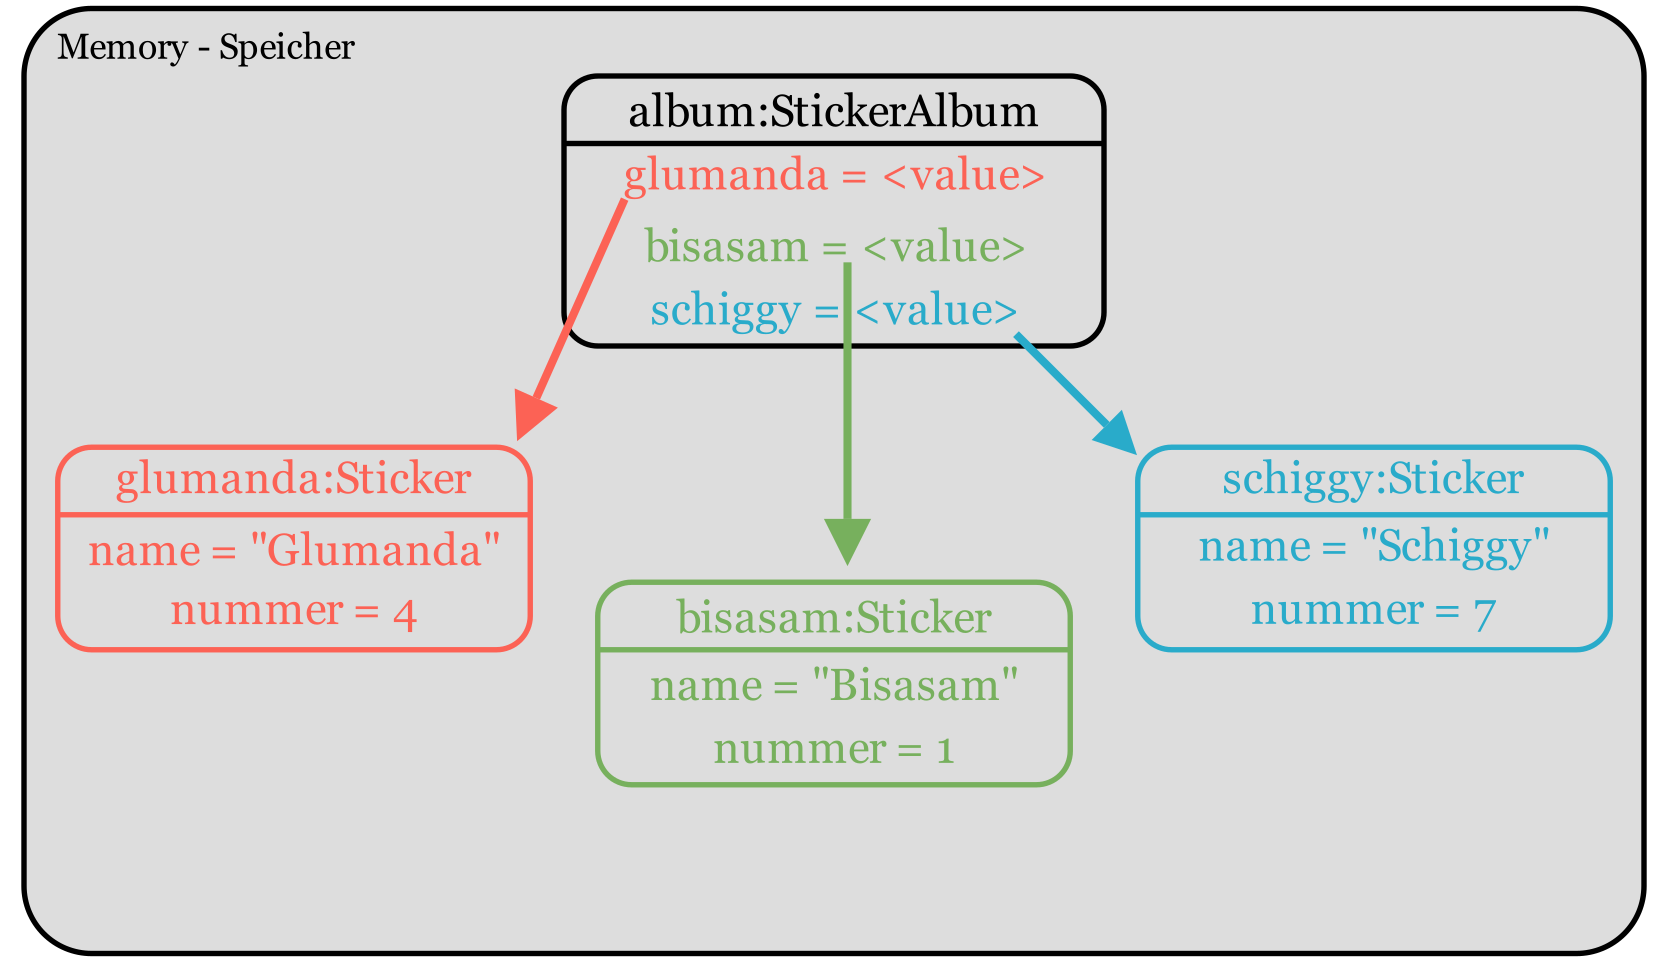
\includegraphics[scale=0.15]{media/speicher_sticker.png}
\end{center}
Ähnliches gilt auch für Arrays. Speichert man primitive Datentypen (also z.B. int, boolean, etc.) in einem Array, so ist die Variable eine Referenz in den Speicher, die an die erste Stelle mit Metadaten zeigt (z.B. liegt dort der Wert des length-Attributs, das wir schon verwendet haben). Anschließend liegen in den folgenden Speicherzellen die Werte explizit abgespeichert. Handelt es sich jedoch um ein Array von Objekten, so ist in jeder der folgenden Speicherzellen nur eine Referenz auf den Speicherort der jeweiligen Objekte vermerkt.
Wären in unserem StickerAlbum von oben die Sticker in einem Array gespeichert, dann sähe Implementierung und Speicherveranschaulichung so aus: 
\begin{minted}{java}
public class StickerAlbum {
    Sticker[] sticker;
    public StickerAlbum() {
        sticker = new Sticker[3];
        sticker[0] = new Sticker(1, "Bisasam");
        sticker[1] = new Sticker(4, "Glumanda");
        sticker[2] = new Sticker(7, "Schiggy");
    }
}
\end{minted}
\begin{center}
    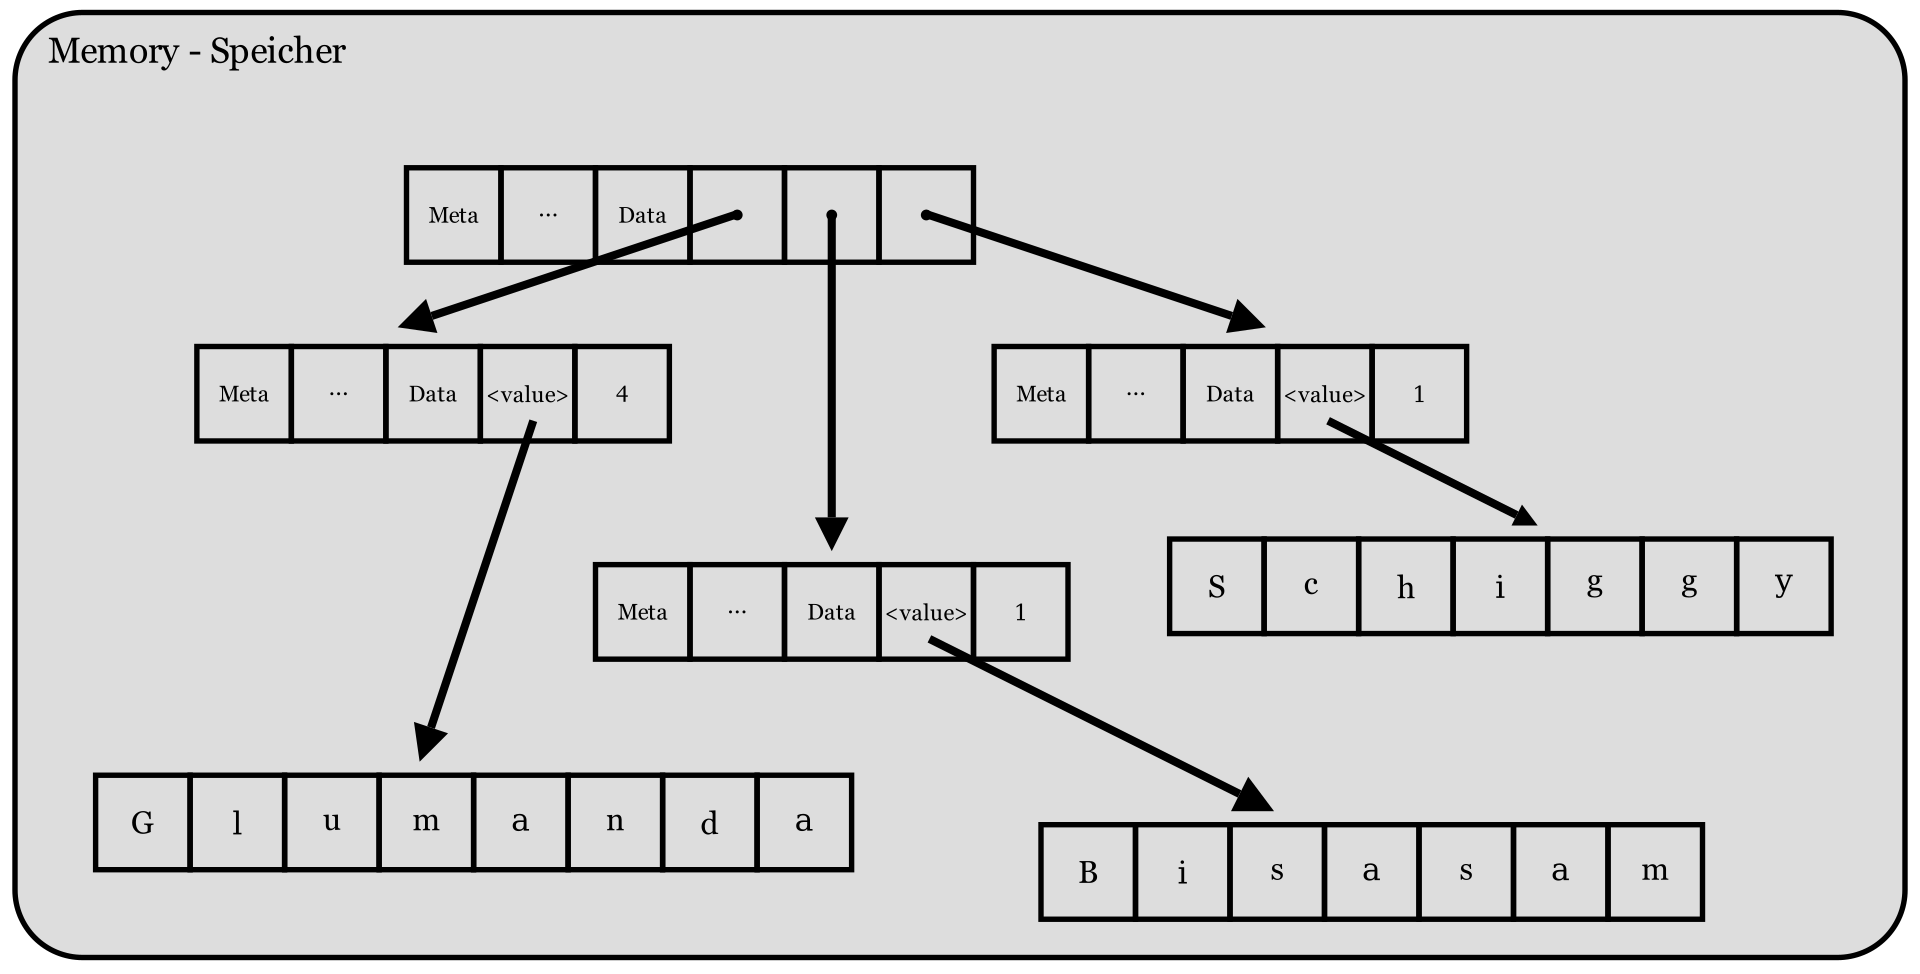
\includegraphics[scale=0.15]{media/speicher.png}
\end{center}
\newpage

Noch einmal zurück zu \textbf{Referenzen}: immer wenn ein Objekt auf ein anderes Objekt \q{verweist} (also nicht nur im Kontext von Arrays) spricht man von einer Referenz. Erst durch diese Referenzen können die Objekte überhaupt miteinander interagieren, da sie ansonsten nichts von der Existenz des jeweils anderen wissen würden. Dabei ergeben sich gewisse Fallstricke. Wir betrachten eine anschauliche Situation, hier als Klassendiagramm:
\begin{center}
    \includegraphics[options]{name}
\end{center} 
\end{document}